\documentclass[a4paper,12pt]{scrartcl}

% Sprach- und Kodierungspakete
\usepackage[utf8]{inputenc}
\usepackage[english,ngerman]{babel}
\usepackage[T1]{fontenc}
\usepackage{graphicx}
\usepackage{expl3,xparse}

% Seitenränder
\usepackage[a4paper,margin=2.5cm,top=80pt,headheight=55pt,headsep=10pt,footskip=35pt]{geometry}

% Zeilenabstand
%\usepackage{setspace}
\usepackage[onehalfspacing]{setspace}
\usepackage{array}

\usepackage[colorlinks=true,linkcolor=black,urlcolor=blue,citecolor=black]{hyperref}
\usepackage{url}
\usepackage[nolinks]{qrcode}

\usepackage[printonlyused]{acronym}
\usepackage{tabularx}
\usepackage{tablefootnote}
\usepackage{multirow}
\usepackage{wrapfig}
\usepackage{threeparttable}
\usepackage[table]{xcolor}
\usepackage{tikz}
\usepackage{microtype}
\usepackage{svg}
\usepackage{pifont}

\usepackage{caption}

\usepackage{enumitem}
\setlist[itemize]{itemsep=0.025em}

\usepackage{csquotes}
\usepackage[style=apa, backend=biber]{biblatex}
\addbibresource{./literature.bib}

\usepackage[l3]{csvsimple}

\newif\ifheader
\newif\iffooter

\newif\iflistoffigurespage
\newif\iflistoftablespage

\newif\iftitlepage
\newif\iftitlepageqrcode
\newif\ifblankpageaftertitlepage

\newif\ifsoftwarepage
    \newif\ifsoftwarepagelineartechnology
    \newif\ifsoftwarepagemicrochipstudio
    \newif\ifsoftwarepagefreecad
    \newif\ifsoftwarepagekicad
    \newif\ifsoftwarepagedremeldigilabslicer

\headerfalse
\footerfalse

\listoffigurespagefalse
\listoftablespagefalse

\titlepagefalse
    \titlepageqrcodefalse
    \blankpageaftertitlepagefalse


\softwarepagefalse
    \softwarepagelineartechnologyfalse
    \softwarepagemicrochipstudiofalse
    \softwarepagefreecadfalse
    \softwarepagekicadfalse
    \softwarepagedremeldigilabslicerfalse

\usepackage{listings}

% Globale Parameter
\setlength{\parindent}{0pt} % Kein Einrücken am Anfang eines Absatzes
\newcommand{\documentAuthor}{R. GÄCHTER}

% Header-Parameter
\headertrue           % Header aktivieren
  \newcommand{\headerLogo}{./images/htl.png}

% Footer-Parameter
\footertrue           % Footer aktivieren
  \newcommand{\footerAuthor}{\documentAuthor}
  \newcommand{\footerVersion}{1.0}

% Page-Parameter
% \acronymspagetrue         % Acronyme aktivieren
% \tableofcontentspagetrue  % Inhaltsverzeichnis aktivieren
\listoffigurespagetrue    % Abbildungsverzeichnis aktivieren
\listoftablespagetrue     % Tabellenverzeichnis aktivieren
% \bibliographypagetrue     % Literaturverzeichnis aktivieren

% Titlepage-Parameter
\titlepagetrue                  % Titelblatt aktivieren
\titlepageqrcodetrue            % QR-Code auf dem Titelblatt aktivieren
% \blankpageaftertitlepagetrue  % Leerseite nach dem Titelblatt aktivieren
  \newcommand{\titleHeadline}{RCC - RGB LED Color Cube}
  \newcommand{\titleLogo}{./images/assembled.png}
  \newcommand{\titleLogoWidth}{0.35}
  \newcommand{\titleRepository}{https://github.com/0x007e/rcc}

% Softwarepage-Parameter
\softwarepagetrue     % Software-Seite aktivieren
  % \softwarepagelineartechnologytrue
  \softwarepagemicrochipstudiotrue
  \softwarepagefreecadtrue
  \softwarepagekicadtrue
  % \softwarepagedremeldigilabslicertrue

% Feste Breite für Tabellen
\renewcommand{\tabularxcolumn}[1]{m{#1}}
\newcolumntype{P}[1]{>{\raggedright\arraybackslash}p{#1}}
\newcolumntype{Y}{>{\raggedright\arraybackslash}X}
\newcolumntype{M}[1]{>{\centering\arraybackslash}m{#1}}
\newcolumntype{N}[1]{>{\raggedright\arraybackslash}m{#1}}
\input{./preamble/commands.tex}

\ifheader
  % Paket für Kopf- und Fußzeilen
\usepackage[automark,headsepline=0.4pt:1.0\textwidth,footsepline=0.4pt:1.0\textwidth]{scrlayer-scrpage}
% Paket für Gesamtseitenzahl
\usepackage{lastpage}

\pagestyle{scrheadings}     % Kopf- und Fußzeilen-Stil setzen

% Standard-Stile von Kopf- und Fußzeilen entfernen
\clearpairofpagestyles

\ihead{\includegraphics[height=1.25cm]{\headerLogo}}
\chead{}
\ohead{
  \parbox[t]{15cm}{
    \raggedleft
    \headerText
  }
}

\fi

\iffooter
  \ifoot{\footerAuthor}
\cfoot{\footerVersion}
\ofoot{\thepage{} / \pageref{LastPage}}

\fi

% ##########################################################################

\begin{document}

% \selectlanguage{ngerman}
% \selectlanguage{english}

\renewcommand{\tablename}{Tab.}

\iflanguage{ngerman}{
  \renewcommand{\figurename}{Abb.}
  
\newcommand{\headerText}{\textbf{HTL-Rankweil}\\\texttt{Abteilung für Elektronik/Informatik}}
\newcommand{\titleLogoCaption}{Zusammengesetzter Cube}
\newcommand{\titleDescription}{\small Das RCC-Projekt basiert auf einer Platine mit einem ATtiny402 und zwei RGB-LEDs, die über den SPI-Bus gesteuert werden. Der Cube selbst wird über einen einzigen Taster gesteuert, der den Cube ein- und ausschaltet und zur Einrichtung der Farbe und Helligkeit der LEDs verwendet werden kann.\\}

\newcommand{\globalimportanttext}{Wichtig:}

\newcommand{\abstracttitle}{Einleitung}
\newcommand{\abstracttext}{
Das \texttt{RCC} (RGB LED Color Cube) Projekt ist ein eingebettetes System, das auf einer PCB mit einem \texttt{ATtiny402}\footnote{\url{https://link.sunriax.at/MecTz}} Mikrocontroller basiert, der zwei RGB-LEDs\footnote{\url{https://link.sunriax.at/nBUNH}} über SPI-Kommunikation steuert. Das System verfügt über eine Benutzeroberfläche mit einem einzigen Taster, um den Cube ein- und auszuschalten und die Farbe sowie die Helligkeitseinstellungen anzupassen. Es umfasst umfassende Hardware-Designs, Firmware und Bibliotheken für eine einfache Integration und Anpassung. Das Projekt nutzt KiCAD für das PCB-Design, FreeCAD für das Gehäuse und Microchip Studio für die Firmware-Entwicklung und legt dabei Wert auf Modularität und professionelle Produktionsbereitschaft durch automatisierte Build-Prozesse mit GitHub Actions. Dieses Setup bietet eine kompakte, vielseitige und programmierbare RGB-Beleuchtungslösung, die sich für Prototyping und Bildungszwecke in der Entwicklung von Elektronik- und eingebetteten Systemen eignet.
\newline
Die Montage der PCB erfolgt mit einer halbautomatischen Bestückungsmaschine, um eine präzise und effiziente Bauteilmontage sicherzustellen. Das Löten der PCB-Bauteile erfolgt mit einem Vapor-Phase-Lötverfahren, das eine gleichmäßige Wärmeverteilung und hochwertige Lötverbindungen gewährleistet. Der Batteriefach wird manuell mit herkömmlichen Lötmethoden verlötet, um eine sorgfältige Handhabung dieses spezifischen Bauteils zu ermöglichen. Das Gehäuse wird durch 3D-Druck hergestellt, was eine schnelle Prototypenerstellung mit hoher Genauigkeit und feinen Details ermöglicht. Darüber hinaus wird die Acrylplatte auf der Unterseite des Gehäuses mit einem CO\textsubscript{2} Laser Cutter zugeschnitten und graviert, um präzise Formen und individuelle Oberflächenmarkierungen zu gewährleisten.
\newline
Dieser Prozess garantiert ein professionell montiertes und fertiges Produkt, das automatisierte Fertigungstechniken mit manueller Präzision und fortschrittlichen Fertigungstechnologien kombiniert.
}

\newcommand{\pcbsectiontitle}{PCB Montage}
\newcommand{\pcbfigureassemblytopcaptiontext}{PCB Top-Bearbeitungs- und Montagelayout}
\newcommand{\pcbfigureassemblybottomcaptiontext}{PCB Bottom-Bearbeitungs- und Montagelayout}

\newcommand{\programmersectiontitle}{Firmware-Programmierung}
\newcommand{\programmerfigureprogrammercaptiontext}{Programmer}
\newcommand{\programmerintroductiontext}{Die Verwendung des \texttt{Programmiergeräts} zum Flashen des \texttt{ATtiny402} über die \texttt{UPDI}-Schnittstelle ist unkompliziert. Die erforderliche Software zum Flashen kann über das \texttt{RCC Programming Repository}\footnote{\url{https://github.com/0x007e/rcc_programmer}} heruntergeladen werden. Über die USB-to-UART-Brücke wird die Firmware auf den Mikrocontroller übertragen. Die Anwendung selbst bietet eine einfache Benutzeroberfläche, um die Firmware auf den \texttt{RCC} zu übertragen. Die Farbe und die Intensität der LEDs kann innerhalb der Anwendung angepasst werden, bevor sie auf den \texttt{RCC} übertragen werden.}
\newcommand{\programmertabledownloadlinkstitle}{RCC - Programmier-Software (Windows x64)}
\newcommand{\programmertabledownloadlinksclickoncetext}{ClickOnce-Installer, der automatisch aktualisiert wird, wenn neue Versionen verfügbar sind.}
\newcommand{\programmertabledownloadlinksportabletext}{Portable Version, die ohne Installation ausgeführt werden kann, aber manuell aktualisiert werden muss.}
\newcommand{\programmertabledownloadlinkscaptiontext}{Download-Links}
\newcommand{\programmerfigureinterfacecaptiontext}{Programmierschnittstelle}
\newcommand{\programmertablenoticetext}{Der \textbf{RCC}-Cube wird durch die USB-UART-Brücke (über die \texttt{Pogo}-Pins) mit \texttt{3V3} versorgt und benötigt keine Batterie. Es ist sicherzustellen, dass das \textbf{RCC}-Gerät \textbf{\textcolor{red}{nicht mit Batterie betrieben wird, um Schäden am Gerät zu vermeiden!}}}
\newcommand{\programmertablenoticecaption}{Programmiergerät-Hinweis}
\newcommand{\programmertableselfmadeupdititle}{Verwenden von externen UPDI-Adaptern}
\newcommand{\programmertableselfmadeupditext}{Ein selbstgebauter UPDI-Adapter kann auch innerhalb einer FT232 USB-to-UART-Brücke oder eines ähnlichen Moduls gemäß den Schaltplänen auf der \texttt{UPDI}\footnote{\url{https://github.com/0x007e/updi}}-Projektseite verwendet werden. Die Verbindungsanordnung finden Sie auf der Programmierer-Projektseite\footnote{\url{https://github.com/0x007e/rcc_programmer}} selbst.}
\newcommand{\programmertableselfmadeupdicaption}{UPDI-Adapter-Informationen}

\newcommand{\mechanicalsectiontitle}{Mechanische Montage}
\newcommand{\mechanicalintroductiontext}{Die mechanische Montage erfolgt durch das Zusammenfügen der 3D-gedruckten Gehäuseteile mit der lasergeschnittenen Acrylplatte. Die PCB wird mit den integrierten Montageschrauben im Gehäuse befestigt. Die Batterie muss montiert werden, bevor die PCB im Gehäuse platziert wird.}
\newcommand{\mechanicalsubsectionsteps}{Notwendige Schritte:}
\newcommand{\mechanicalfigurecaptionexplosion}{Explosionsansicht der mechanischen Montage}

\newcommand{\mechanicaltextfile}{./data/mechanicaltext.de.csv}
\newcommand{\mechanicalstepsfile}{./data/mechanicalsteps.de.csv}

}{
  \renewcommand{\figurename}{Fig.}
  
\newcommand{\headerText}{\textbf{HTL-Rankweil}\\\texttt{Department of Electronics/Informatics}}
\newcommand{\titleLogoCaption}{Assembled Cube}
\newcommand{\titleDescription}{\small The RCC project is based on a pcb with an ATtiny402 and two RGB LEDs that are controlled via SPI-bus. The cube itself is controlled over a single push-button that enables/disables the cube and can be used to setup the color and intensity of the leds.\\}

\newcommand{\globalimportanttext}{Important:}

\newcommand{\abstracttitle}{Abstract}
\newcommand{\abstracttext}{
The \texttt{RCC} (RGB LED Color Cube) project is an embedded system based on a PCB with an \texttt{ATtiny402}\footnote{\url{https://link.sunriax.at/MecTz}} microcontroller controlling two RGB LEDs\footnote{\url{https://link.sunriax.at/nBUNH}} via SPI communication. The system features a user interface with a single push-button to toggle the cube and adjust its color and brightness settings. It includes comprehensive hardware designs, firmware, and libraries for easy integration and customization. The project leverages KiCAD for PCB design, FreeCAD for housing, and Microchip Studio for firmware development, emphasizing modularity and professional production readiness through automated build processes using GitHub Actions. This setup provides a compact, versatile, and programmable RGB lighting solution suitable for prototyping and educational purposes in electronic and embedded systems development.
\newline
The assembly of the PCB is carried out using a semi-automatic placement machine to ensure precise and efficient component mounting. Soldering of the PCB components is performed with a vapor phase soldering system, which provides uniform heat distribution and high-quality solder joints. The battery holder is soldered manually using conventional soldering methods to allow for careful handling of this specific component. The enclosure is produced by 3D printing, enabling rapid prototyping with high accuracy and fine detail. Additionally, the acrylic plate on the bottom side of the enclosure is cut and engraved using a CO\textsubscript{2} laser cutter, ensuring precise shaping and custom surface markings.
\newline
This process guarantees a professionally assembled and finished product combining automated manufacturing techniques with manual precision and advanced fabrication technologies.
}

\newcommand{\pcbsectiontitle}{PCB Assembly}
\newcommand{\pcbfigureassemblytopcaptiontext}{PCB Top fabrication and assembly layout}
\newcommand{\pcbfigureassemblybottomcaptiontext}{PCB Bottom fabrication and assembly layout}

\newcommand{\programmersectiontitle}{Firmware programming}
\newcommand{\programmerfigureprogrammercaptiontext}{Programmer}
\newcommand{\programmerintroductiontext}{Using the \texttt{programming tool} to flash the \texttt{ATtiny402} via \texttt{UPDI} interface is straightforward. Just download and install the required software and flash it with the \texttt{RCC Programming Toolkit}\footnote{\url{https://github.com/0x007e/rcc_programmer}} over the implemented USB-to-UART bridge in the \texttt{RCC-Programmer}. The \texttt{programming tool} itself can be installed or used as a portable application. The application itself provides a simple user interface to flash the firmware onto the \texttt{RCC} device. Therefore the color and intensitry of the LEDs can be adjusted within the application before flashing it onto the device.}
\newcommand{\programmertabledownloadlinkstitle}{RCC - Programming Software (Windows x64)}
\newcommand{\programmertabledownloadlinksclickoncetext}{ClickOnce installer that updates automatically when new versions are available.}
\newcommand{\programmertabledownloadlinksportabletext}{Portable version that can be run without installation but needs to be updated manually.}
\newcommand{\programmertabledownloadlinkscaptiontext}{Download Links}
\newcommand{\programmerfigureinterfacecaptiontext}{Programming Interface}
\newcommand{\programmertablenoticetext}{The \textbf{RCC}-Cube is powered through the USB-UART bridge (through the \texttt{Pogo}-pins) with \texttt{3V3} and does not require a battery. It must be ensured that the \textbf{RCC} device is \textbf{\textcolor{red}{not powered by battery to avoid damage to the device!}}}
\newcommand{\programmertablenoticecaption}{Programmer Notice}
\newcommand{\programmertableselfmadeupdititle}{Using of external UPDI-Adapters}
\newcommand{\programmertableselfmadeupditext}{A selfmade UPDI adapter can also be used within an FT232 USB-to-UART bridge or a similar module according to the schematics provided on the \texttt{UPDI}\footnote{\url{https://github.com/0x007e/updi}} project page. The connection setup can be found on the programmer project site\footnote{\url{https://github.com/0x007e/rcc_programmer}} itself.}
\newcommand{\programmertableselfmadeupdicaption}{UPDI-Adapter Information}

\newcommand{\mechanicalsectiontitle}{Mechanical Assembly}
\newcommand{\mechanicalintroductiontext}{The mechanical assembly is done by assembling the 3D printed enclosure parts together with the laser-cut acrylic plate. The PCB is mounted inside the enclosure using the integrated mounting features. The battery has to be mounted before the PCB is placed inside the enclosure.}
\newcommand{\mechanicalsubsectionsteps}{Necessary steps:}
\newcommand{\mechanicalfigurecaptionexplosion}{Exploded view of the mechanical assembly}

\newcommand{\mechanicaltextfile}{./data/mechanicaltext.en.csv}
\newcommand{\mechanicalstepsfile}{./data/mechanicalsteps.en.csv}

}

\iftitlepage
  \newif\ifnotempty

\newcommand{\fieldNotEmpty}[1]{
  \def\temp{#1}%
  \ifx\temp\empty
    \notemptyfalse
  \else
    \notemptytrue
  \fi
}

\begin{titlepage}
	\title{\titleHeadline}
	\subtitle{
    \fieldNotEmpty{\titleLogo}
    \ifnotempty
      \begin{figure}[htb]
          \centering
          \includegraphics[width=\titleLogoWidth\textheight]{\titleLogo}
          \caption{\titleLogoCaption}
          \label{fig:titlepage-image}
      \end{figure}
    \fi
    \fieldNotEmpty{\titleLogo}
    \ifnotempty
      \begin{center}
        \Large \titleDescription
      \end{center}
    \fi
    \fieldNotEmpty{\titleRepository}
    \ifnotempty
      \small Repository:\\
      \begin{center}
          \href{\titleRepository}{\texttt{\titleRepository}}
      \end{center}
      \iftitlepageqrcode
        \qrcode[height=1in]{\titleRepository}
      \fi
    \fi
  }
	\author{\small \documentAuthor}
	\date{\small \today}
	\thispagestyle{empty}
\end{titlepage}
  \maketitle

  \thispagestyle{empty}
  \newpage

  \ifblankpageaftertitlepage
    ~
    \thispagestyle{empty}
    \newpage
  \fi
\fi

\ifsoftwarepage
  \newcounter{softwaretnotecounter}

\iflanguage{ngerman}{
  \newcommand{\softwaresectiontitle}{Verwendete Software}
  \newcommand{\softwaretableimage}{Abbildung}
  \newcommand{\softwaretablename}{Name}
  \newcommand{\softwaretabledescription}{Beschreibung}
  \newcommand{\softwaretablecaptiontext}{Softwarekomponenten für das Projekt}

  \newcommand{\softwareltspicetext}{Simulationssoftware für elektronische Schaltungen, weitverbreitet zum Entwurf und Testen von Schaltungen.}
  \newcommand{\softwaremicrochipstudiotext}{Entwicklungsumgebung (IDE) zur Programmierung von Mikrocontrollern, insbesondere AVR und ARM.}
  \newcommand{\softwarefreecadtext}{Open-Source CAD-Software für 3D-Modellierung, geeignet für technische Konstruktionen und Design.}
  \newcommand{\softwarekicadtext}{Open-Source PCB-Design-Software, geeignet für die Erstellung von Leiterplattenlayouts.}
  \newcommand{\softwaredremeldigilabslicertext}{Software zum Vorbereiten und Slicen von 3D-Druck-Modellen, speziell für Dremel 3D-Drucker optimiert.}

  \newcommand{\softwarelogotext}{Die abgebildeten Logos sind markenrechtlich geschützte Symbole. Sie werden in dieser Dokumentation ausschließlich zur Identifikation der jeweiligen Softwareprodukte verwendet, ohne Werbeabsicht.}
}{
  \newcommand{\softwaresectiontitle}{Used Software}
  \newcommand{\softwaretableimage}{Figure}
  \newcommand{\softwaretablename}{Name}
  \newcommand{\softwaretabledescription}{Description}
  \newcommand{\softwaretablecaptiontext}{Software components for the project}

  \newcommand{\softwareltspicetext}{Simulation software for electronic circuits, widely used for designing and testing circuits.}
  \newcommand{\softwaremicrochipstudiotext}{Development environment (IDE) for programming microcontrollers, especially AVR and ARM.}
  \newcommand{\softwarefreecadtext}{Open-source CAD software for 3D modeling, suitable for technical constructions and design.}
  \newcommand{\softwarekicadtext}{Open-source PCB design software, suitable for creating printed circuit board layouts.}
  \newcommand{\softwaredremeldigilabslicertext}{Software for preparing and slicing 3D print models, specifically optimized for Dremel 3D printers.}

  \newcommand{\softwarelogotext}{The logos shown are protected by trademark law. They are used in this documentation solely for the identification of the respective software products, without any advertising intent.}
}

\section*{\softwaresectiontitle}
\begin{table}[!ht]
  \renewcommand{\arraystretch}{1.3}
  \centering
  \begin{threeparttable}
    \begin{tabularx}{\linewidth}{|M{2.4cm}|M{2.2cm}|X|}
      \hline
      \rowcolor{gray!20}
      \textbf{\softwaretableimage\tnote{*}} & \textbf{\softwaretablename} & \textbf{\softwaretabledescription} \\
      \hline
\ifsoftwarepagelineartechnology
      \stepcounter{softwaretnotecounter}
      \raisebox{-.25\height}{\includesvg[width=1.6cm,inkscapelatex=false]{./logo/linear_technology}} &
      LT-Spice\tnote{(\thesoftwaretnotecounter)} &
      \softwareltspicetext\\
      \hline
\fi
\ifsoftwarepagemicrochipstudio
      \stepcounter{softwaretnotecounter}
      \raisebox{-.25\height}{\includesvg[width=1.6cm,inkscapelatex=false]{./logo/microchip}} &
      Microchip Studio\tnote{(\thesoftwaretnotecounter)} &
      \softwaremicrochipstudiotext\\
      \hline
\fi
\ifsoftwarepagefreecad
      \stepcounter{softwaretnotecounter}
      \raisebox{-.25\height}{\includesvg[width=0.65cm,inkscapelatex=false]{./logo/freecad}} &
      FreeCAD\tnote{(\thesoftwaretnotecounter)} &
      \softwarefreecadtext\\
      \hline
\fi
\ifsoftwarepagekicad
      \stepcounter{softwaretnotecounter}
      \raisebox{-.25\height}{\includesvg[width=0.65cm,inkscapelatex=false]{./logo/kicad}} &
      KiCAD\tnote{(\thesoftwaretnotecounter)} &
      \softwarekicadtext\\
      \hline
\fi
\ifsoftwarepagedremeldigilabslicer
      \stepcounter{softwaretnotecounter}
      \raisebox{-.25\height}{\includesvg[width=1.6cm,inkscapelatex=false]{./logo/dremel}} &
      Dremel 3D DigiLab Slicer\tnote{(\thesoftwaretnotecounter)} &
      \softwaredremeldigilabslicertext\\
      \hline
\fi
    \end{tabularx}
    \caption{\softwaretablecaptiontext}
    \label{tab:software-programme}
    \begin{tablenotes}
      \footnotesize
      \item[*] \softwarelogotext
      \item[~]
\setcounter{softwaretnotecounter}{0}
\ifsoftwarepagelineartechnology
      \stepcounter{softwaretnotecounter}
      \item[(\thesoftwaretnotecounter)] \url{https://www.analog.com/en/resources/design-tools-and-calculators.html}
\fi
\ifsoftwarepagemicrochipstudio
      \stepcounter{softwaretnotecounter}
      \item[(\thesoftwaretnotecounter)] \url{https://www.microchip.com/en-us/tools-resources/develop/microchip-studio}
\fi
\ifsoftwarepagefreecad
      \stepcounter{softwaretnotecounter}
      \item[(\thesoftwaretnotecounter)] \url{https://www.freecad.org/downloads.php}
\fi
\ifsoftwarepagekicad
      \stepcounter{softwaretnotecounter}
      \item[(\thesoftwaretnotecounter)] \url{https://www.kicad.org/download/}
\fi
\ifsoftwarepagedremeldigilabslicer
      \stepcounter{softwaretnotecounter}
      \item[(\thesoftwaretnotecounter)] \url{https://www.dremel.com/at/de/digilab/3d-druckersoftware}  
\fi
    \end{tablenotes}
  \end{threeparttable}
\end{table}

  \thispagestyle{empty}
  \newpage
\fi

\section*{\abstracttitle}
\abstracttext

\thispagestyle{empty}
\newpage

\setcounter{page}{1}

\noindent\hfill\texttt{GAR@\today|\jobname.pdf}
\vspace{-25pt}

\section{\pcbsectiontitle}

\begin{figure}[!htbp]
  \vspace{-20pt}
  \centering
  \includegraphics[page=5, angle=90, scale=0.77, trim=20pt 20pt 20pt 20pt, clip]{pcb.pdf}
  \caption{\pcbfigureassemblytopcaptiontext}
  \label{fig:pcb-top-assembly}
\end{figure}
\newpage

\begin{figure}[!htbp]
  \centering
  \includegraphics[page=6, angle=90, scale=0.77, trim=20pt 20pt 20pt 20pt, clip]{pcb.pdf}
  \caption{\pcbfigureassemblybottomcaptiontext}
  \label{fig:pcb-bottom-assembly}
\end{figure}
\newpage

\section{\programmersectiontitle}

\begin{wrapfigure}{r}{0.25\textwidth}
  \vspace{-50pt}
  \includegraphics[width=\linewidth]{./images/programmer_assembled.png}
  \caption{\programmerfigureprogrammercaptiontext}
  \label{fig:rcc-programmer-image}
\end{wrapfigure}

\programmerintroductiontext

\begin{table}[!htbp]
  \renewcommand{\arraystretch}{1.2}
  \noindent
  \begin{minipage}{\textwidth}
    \begin{tabularx}{\textwidth}{|c|c|X|}
      \hline
      \rowcolor{gray!20}
      \multicolumn{3}{|c|}{\textbf{\programmertabledownloadlinkstitle}} \\
      \hline
      \multirow{2}{*}{
        \raisebox{-.5\height}{
          \includegraphics[height=1.35cm]{./images/programmer_icon.png}
        }
      } & 
      \href{https://0x007e.github.io/rcc_programmer/clickonce/setup.exe}{\textbf{Installer}}\footnote{\url{https://0x007e.github.io/rcc_programmer/clickonce/setup.exe}} &
      \programmertabledownloadlinksclickoncetext \\
      \cline{2-3}
       & \href{https://github.com/0x007E/rcc_programmer/releases/latest/download/programmer.zip}{\textbf{Portable}}\footnote{\url{https://github.com/0x007E/rcc_programmer/releases/latest/download/programmer.zip}} &
      \programmertabledownloadlinksportabletext \\
      \hline
    \end{tabularx}
    \caption{\programmertabledownloadlinkscaptiontext}
    \label{tab:rcc-programming-download-links}
  \end{minipage}
\end{table}

\vspace{-15pt}
\begin{table}[!htbp]
  \renewcommand{\arraystretch}{1.2}
  \noindent
  \begin{minipage}[t]{0.55\textwidth}
    \vspace{0pt}
    \centering
    \includegraphics[width=\textwidth]{./images/programmer_program.png}
    \caption{\programmerfigureinterfacecaptiontext}
    \label{fig:rcc-programming-interface}
  \end{minipage}%
  \hfill
  \begin{minipage}[t]{0.42\textwidth}
    \vspace{0pt}
    \centering
    \begin{tabularx}{\textwidth}{|M{0.85cm}|X|}
      \hline
      \rowcolor{gray!20}
      \raisebox{-.25\height}{\includesvg[height=0.55cm,inkscapelatex=false]{./symbol/warning}} & \textbf{\globalimportanttext} \\
      \hline
      \multicolumn{2}{|p{\dimexpr\textwidth-2\tabcolsep}|}{\programmertablenoticetext} \\
      \hline
    \end{tabularx}
    \caption{\programmertablenoticecaption}
    \label{tab:rcc-programmer-notice}
  \end{minipage}
\end{table}

\vspace{-10pt}
\begin{table}[!ht]
  \renewcommand{\arraystretch}{1.2}
  \centering
  \begin{tabularx}{\textwidth}{|M{0.85cm}|X|}
      \hline
      \rowcolor{gray!20}
      \raisebox{-.25\height}{\includesvg[height=0.55cm,inkscapelatex=false]{./symbol/info}} & \textbf{\programmertableselfmadeupdititle} \\
      \hline
      \multicolumn{2}{|p{\dimexpr\textwidth-2\tabcolsep}|}{\programmertableselfmadeupditext} \\
  \hline
  \end{tabularx}
  \caption{\programmertableselfmadeupdicaption}
  \label{tab:rcc-programmer-selfmade-updi}
\end{table}

\newpage

\section{\mechanicalsectiontitle}
\mechanicalintroductiontext
\subsection*{\mechanicalsubsectionsteps}

\begin{itemize}
  \setlength\itemsep{-5pt}
  \setlength\parskip{5pt}
  \csvreader[head to column names]{\mechanicalstepsfile}{}
  {
    \item \itemtext
  }
\end{itemize}

\begin{figure}[htb]
  \vspace{-15pt}
  \centering
  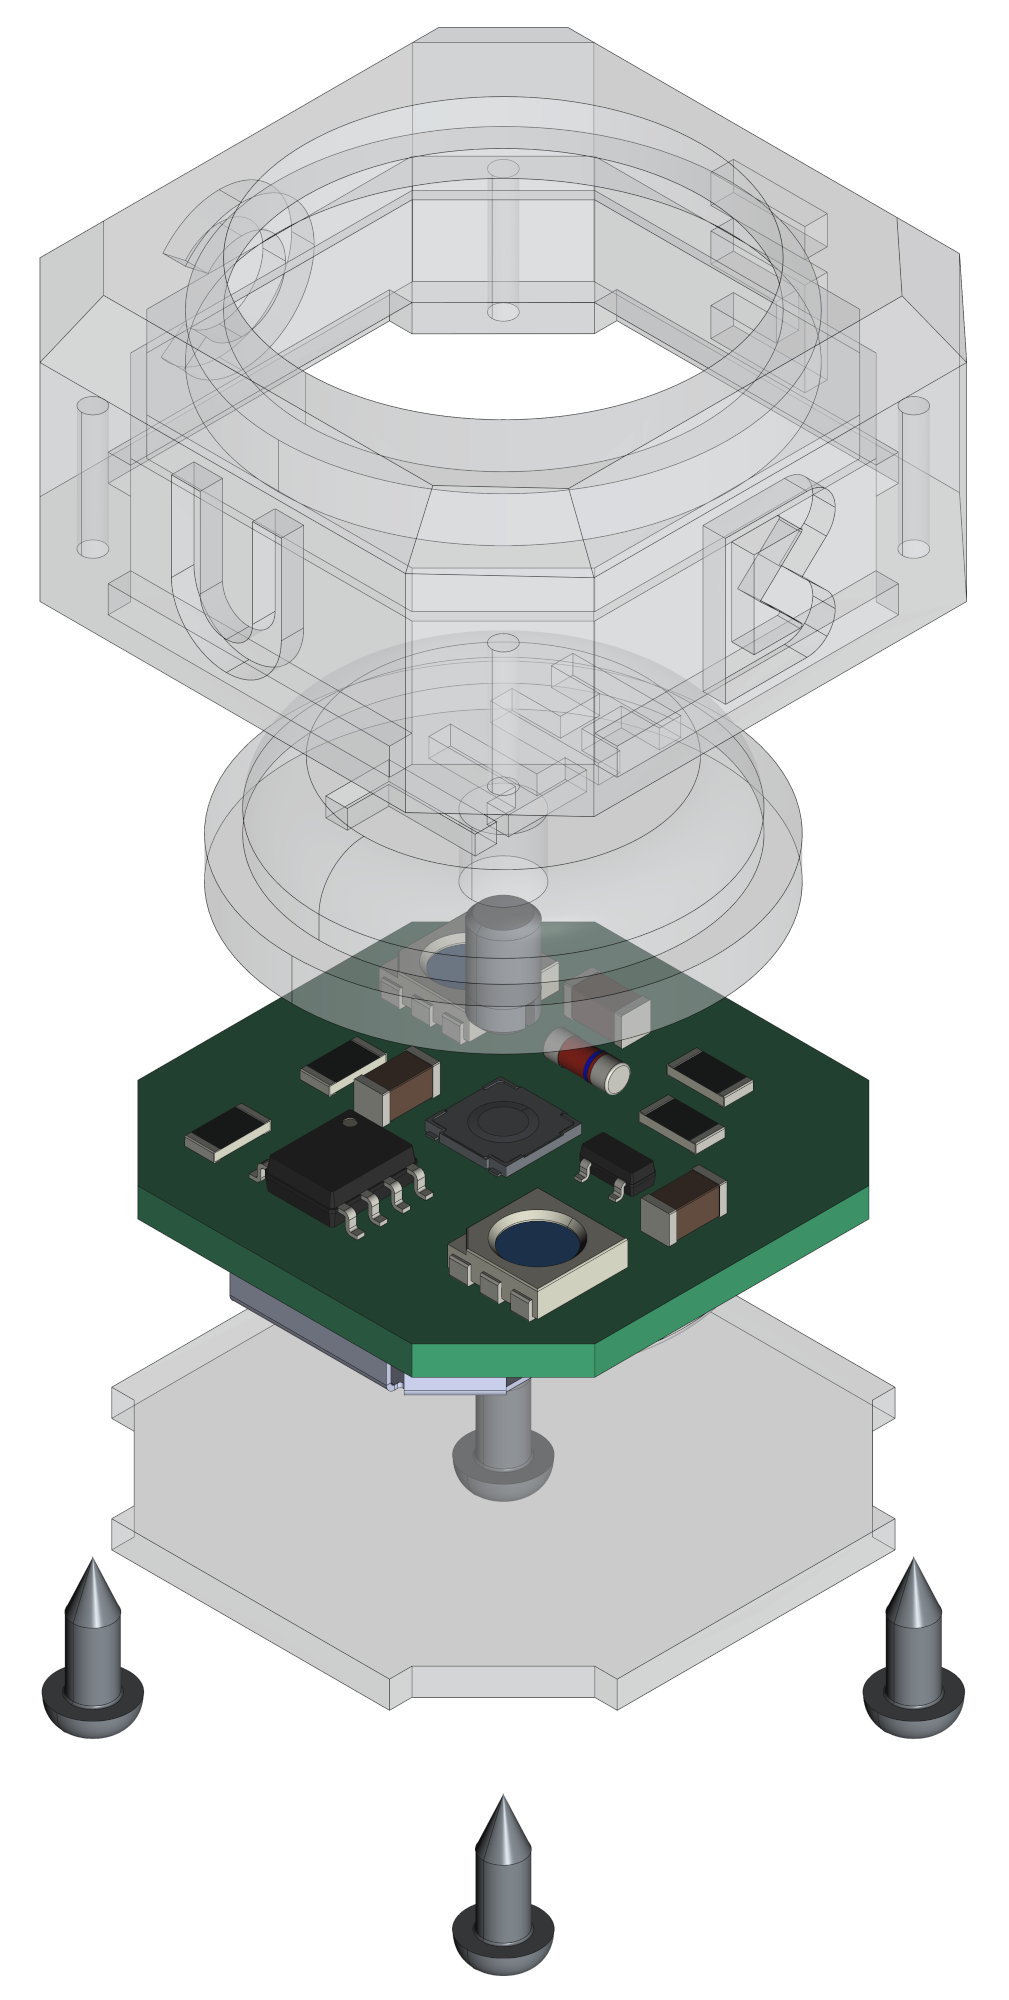
\includegraphics[width=0.4\textwidth]{./images/explosion.png}
  \caption{\mechanicalfigurecaptionexplosion}
  \label{fig:mechanical-explosion}
\end{figure}
\newpage

\iflistoffigurespage
  \listoffigures
\fi

\iflistoftablespage
  \listoftables
\fi

\iflistoffigurespage
  \thispagestyle{empty}
  \newpage
\else
  \iflistoftablespage
    \thispagestyle{empty}
    \newpage
  \fi
\fi

\end{document}